\section{Region of Interest}

With respect to different seismicity rates of the regions \citep{Nemati2015}, as well as the completeness of the seismic catalog \citep{Zare2014} , the study region is divided into three tectonic seismic zones. Each of these zones is characterized by its respective seismicity parameters values, including b-value and maximum magnitude ($M{_{max}}$). Part of Central Iran and Zagros regions are inside of the study region. We also calculated the seismicity parameters in these regions. Fig.~\ref{fig:Iran} shows the study region and different seismotectonic classification.

\begin{figure*}[!ht] 
\centering
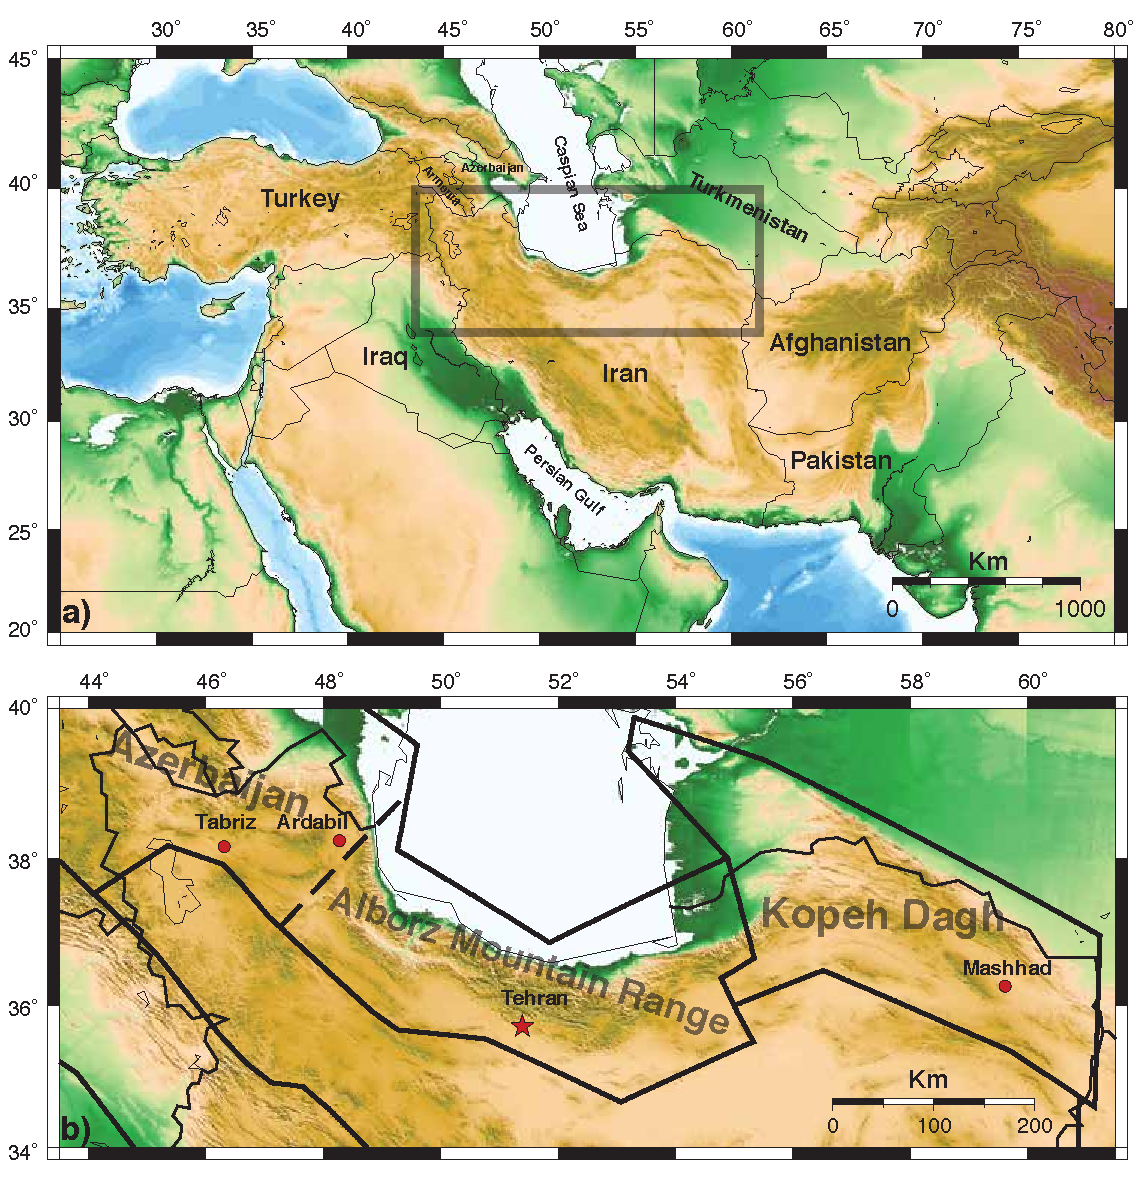
\includegraphics[scale=0.7]{figures/pdf/Figure1.pdf} 
\caption{ a) Map of Iran and surrounding countries. The study area is presented in gray box. b) The study area containing seismotectonic provinces after \citet{Mirzaei1998}, and location of big cities. Dashed line is the subdivision that is proposed by \citet{Karimiparidari2013}. }
 
\label{fig:Iran}
\end{figure*}

\subsection{Tectonic Regions and Seismic Faults}

\subsubsection{Alborz Mountain Range (Alborz)}
Tehran region has active reverse faults, which are parallel to the northwest-trending structural gain of the Alborz Mountains belt. Here a series of historical earthquakes occurred within a time period of more than 1100 years. Four earthquakes with magnitude more than 7 devastated the Tehran region in four centuries period, from 743 to 1177, but in the last 800 years, only one earthquake at 1830 has struck this region. At least three damaging earthquakes in 958 (western segments), 1655 (eastern segments), and 1830 (central segments), ruptured adjacent segments of the Mosha fault, located in northern Tehran.
The North Tehran Thrust (NTT) adds more complexity due to the presence of south-dipping reverse faults, which are in part blind, such as the Davudieh, Shian, and Bagh-E Feyz.
The northwest continuation of the Alborz Mountains, known as the Rocks of the Talesh Mountains, have been thrust northeastward and eastward over rocks of the south Caspian depression. An earthquake with Ms 6.0 in 1978 led to a focal mechanism consistent with a low-angle thrust \citep{Berberian1999}. Recently, the 1990 $M_w$ 7.4 Manjil-Rudbar earthquake caused extensive loss of life and significant damage \citep{USGS_manjil}. Based on existing documents, Tehran city and ancient Rey city have been destroyed completely several times by severe earthquakes with magnitudes greater than 7 \citep{Ambraseys2005}. \\

\subsubsection{Azerbaijan}
There were three earthquakes from 1721-86 that ruptured the North Tabriz Fault system from southeast to northwest. The Tabriz region is in the Araxes structural block of northwestern Iran, southwest of the continuation of the western Alborz Mountains towards the Caucasus. The North Tabriz Fault (NTF) is a complex northwest-trending structure, which contains evidence observed on aerial photographs, and vertical displacement with the north side up, of right-lateral strike-slip displacement \citep{Berberian1999}.
The NTF system and nearby reverse faults ruptured from southeast to northwest in three earthquakes over 65 years: the Shebli earthquake with magnitude 7.3 in 1721 on the southeastern NTF with a surface rupture more than 35 km long, reported by \citet{Jones1834} the Tabriz earthquake with magnitude 7.4 in 1780 on the northwestern NTF, with a surface rupture more than 42 km long and vertical separation of 2 to 4 $m$; and the Marand-Mishu earthquake with magnitude of 6.3 in 1786 on the Mishu reverse fault and the Sufian segment of the NTF. Another earthquake with  magnitude 5.5 struck the Tasuj reverse fault farther west in 1807 and an earthquake of M 6.7 took place along the South Bozqush reverse fault farther southeast in 1879. Prior to the 1721-86 earthquake sequence, Tabriz was shaken by earthquakes in 858 (M 6.0), 1042 (M 7.3), 1273 (M ~ 6.5), and 1304 (M 6.7)\citep{Berberian1999}. Most recently, earthquakes with $M_w$ 6.1 in 1997 and $M_w$ 6.4 in 2012 occurred in Ardabil and Tabriz, respectively. These earthquakes caused around 1500 casualties and extensive damage \citep{USGS_ardabil,USGS_tabriz}.\\


\subsubsection{Kopeh Dagh}
The main Kopeh-Dagh fault system has experienced some historic earthquakes. Ashgabat, the capital city of Turkmenistan, was destroyed by an earthquake of Ms 7.2 in 1948 and destroyed more than 30 villages in Iran. This was the strongest earthquake to strike this region since at least 1455.
The main Kopeh-Dagh fault consists of several partly overlapping segments parallel to the overall $NW - SE$ structure with step-overs. The regions of overlap are characterized by shorter south-dipping thrust faults striking about $E - W$ \citep{Berberian2001}. \citet{Trifonov1978} reported active displacement along the main Kopeh-Dagh fault for more than 500 km. 
Massive destruction of the capital city of Mithradatkert is attributed to the 10 BC event Ms 7.1, roughly 30 kilometers from the border of Iran (Nesa mound) \citep{Berberian2001}.
The Neyshabur sequence of four earthquakes between 1209 and 1405 respected the segment boundary between the Neyshabur and Binalud reverse fault system \citep{Berberian1999}.
Historical records show that in 1209, the district of Neyshabur from Neyshabur city in the west to Daneh village in the east was totally destroyed \citep{Berberian1999}.\\



\subsection{Historical  and Instrumental Seismicity}
Uniform earthquake catalog is the most important factor in seismic hazard analysis of a region.  Different studies have been conducted in order to prepare a uniform catalog for Iranian Earthquake. Historical event interpretation and different magnitude conversion relationships are some of the factors which make all these catalogs different. Among different sources \citet{Ambraseys2005}, \citet{Berberian1994}, and \citet{moinfar1994} are some of the main sources for Iranian earthquake catalog. These catalogs contain historical and instrumental earthquakes that have been reported in literature and national and international networks. According to \citet{Ambraseys2005}, there are some scattered indication of earthquake effects  back to third millinuim BC. However, adequate documentary coverage of individual events begins from seventh century A.D. \citet{Mirzaei1997} provided a comprehensive list of studies that have been done in compilation a uniform catalog for Iranian earthquakes in order to prepare a uniform catalog of earthquake (all earthquakes are converted to surface wave magnitude Ms) for seismic hazard assessment in Iran. The catalog is covering the period of 4th century B.C. through 1994. The instrumental data is achievable from three national agencies including IIEES, International Institute of Earthquake Engineering and Seismology; IRSC, The Iranian seismological center, University of Tehran; and BHRC, Building and Housing Research Center (Iran Strong Motion Network) (For more information about these networks see \citet{Karimiparidari2013}).
Many most of attenuation relationship use  moment magnitude $M_w$ as an input for the equation \citep{Douglas2011}. Moment magnitude is not suffering from saturation and has physical meaning \citep{Kanamori1977}. Due to mentioned reasons Mw has become a most appropriate magnitude scale in recent studies. 
 \citet{Karimiparidari2013}compiled a uniform earthquake catalog for Iran and adjacent areas, using international and national databanks until April 2010.  They developed relationships between moment magnitude and other magnitude based on orthogonal regression.  They removed the dependent events (aftershocks and foreshocks) using the procedure by \citet{Gardner1974}. The catalog of events with magnitude equal and above Mw 5.5 is provided. 
\citet{Shahvar2013} presented a unified and homogeneous catalog for the Iranian plateau $(M_w >= 4)$, created by merging data from two local catalogs and seven international agencies for 1900-2011 period. They used orthogonal regression method \citep{Castellaro2006} to derive magnitude conversion relation. By removing foreshocks and aftershocks according to the procedure detailed in Uhrhammer(1986), they also provided declustered version of the catalog.

The recent unified catalog for Middle East region is published as a part of Global Earth Model (GEM) and the Earthquake Model of the Middle East (EMME) project by \citet{Zare2014}. They used all historical (pre-1900), early and modern instrumental events up to 2006. The catalog contains data from Alborz-Azerbaijan, Afghanistan-Pakistan, Saudi Arabia, Caucasus, Central Iran, Kopeh-Dagh, Makran, Zagros, and part of Turkey. The magnitude of all events are converted to Mw through relationships which is derived at previous studies or newly derived at the study relationships. They declustered data through different methods including \citet{Gardner1974}, Uhrhammer(1986), \citet{Reasenberg1985}, and Gruenthal. \citet{Zare2014} provided the catalog completeness for different magnitude range using  the cumulative frequency-magnitude distribution of  \citet{Gutenberg1944} and \citet{richter1958}, and frequency magnitude distributaion of ZMAP \citep{Wiemer2001} software. The methods confirms the results of each other. 

In this study we consider earthquakes with Mw equal and greater than 3. Earthquakes with magnitude 3 are not considered as a structural threat, however, the epicenter of earthquakes with magnitude $M_w 3$ are a  susceptible location for future bigger earthquakes.  According to our preliminary data processing based on IIEES data, Iranian catalog for earthquake with magnitude greater and equal 3, is complete from 2005. In order to make sure about the completeness of the catalog, we use IIEES data from 2000. We used the EMME project data provided by \citet{Zare2014} up to 2000. Fig.~\ref{fig:historical} represents the historical data (pre 1900) in the study region. 

\subsubsection{Magnitude Conversion}

The catalog of recorded earthquake from 2000-2015 which is downloaded from IIEES is reported the earthquake based on different magnitude scale. We converted the $M_L$, $M_s$, and $mb$ magnitudes through conversion relationships which is defined in \citet{Zare2014}. There also some of data which is recorded in $M_D$ (Duration magnitude). These data are reported by International Seismological Centre (ISC).  \citet{Deniz2010}, developed a set of empirical equations to convert earthquake magnitudes in $mb$, $M_D$, $M_L$ and $M_s$ scales to the $M_w$ scales using orthogonal regression procedure. They used data of earthquake that occurred in Turkey from different data centers including ISC. In this study we use the conversion equation of \citet{Deniz2010} to convert the Md to Mw. Although they defined the equation based on $M_w>=4.5$, we extrapolate the equation for lower magnitude. We believe having those earthquakes, even with small error  in magnitude is important for estimating an accurate "a" value  in Gutenberge-Richter equation.

\begin{figure*}[!ht] 

\centering
\includegraphics[scale=0.4]{figures/pdf/Figure2.pdf} 
\caption{Historical earthquakes of Iran (pre 1900). Different colors represent different year of occurrences and size of circles are proportional to the earthquake magnitude. }
\label{fig:historical}
\end{figure*}


\subsubsection{Declustering}

It is generally assumed that the seismicity of each tectonic seismic source follows a Poissonian occurrence process. Therefore, in order to accomplish this, we declustered the earthquake catalog. In compiling the catalog of events, foreshocks and aftershocks were removed using a declustering methodology \citep{Gardner1974}. For north Iran (lon: 42-62.5, lat: 33-41), from 7478 earthquake event we removed 605 Foreshocks and 2917 aftershocks.
Whole data that we used for seismicity parameters of Zagros and Central Iran tectonic seismic regions are not included in these numbers. Fig.~\ref{fig:instrumental} shows the epicenter of declustered instrumental  earthquakes.


\begin{figure*}[!ht] 

\centering
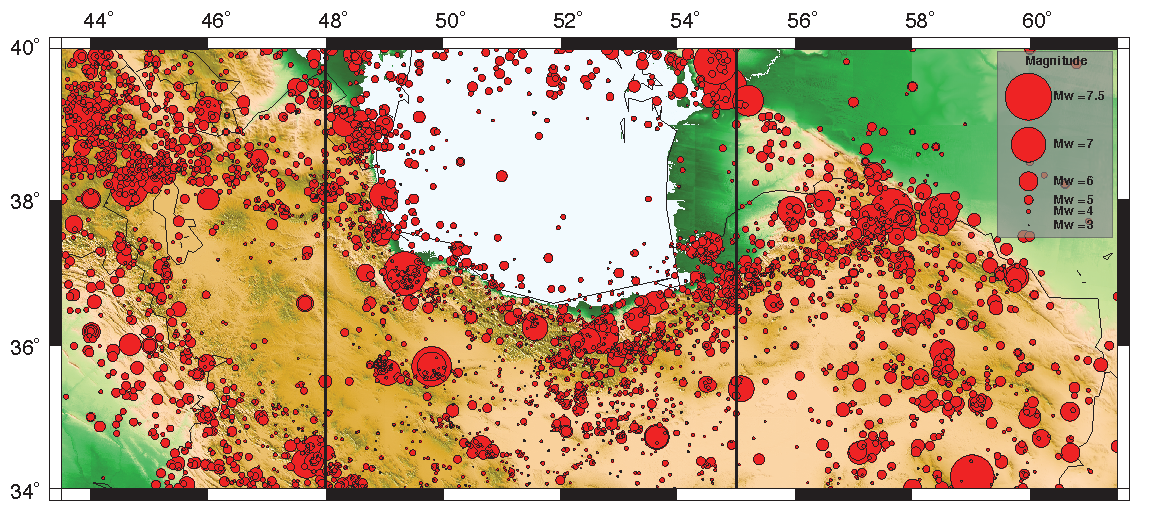
\includegraphics[scale=0.25]{figures/pdf/Figure3.pdf} 
\caption{Declustered instrumental seismicity map (after 1900) of Northern Iran. The study areas are separated at longitude of 48$^{\circ}$ and 55$^{\circ}$ . } 
\label{fig:instrumental}
\end{figure*}


\subsection{Divisions}

As we discussed earlier (see the Introduction section), classifying the tectonic seismic regions has been a controversial debate. In this study we consider two seismic tectonic models. First model is according to \citet{Mirzaei1998} and \citet{Karimiparidari2013} classification, which includes Azerbaijan, Alborz, Kopek Dagh, and part of Central Iran, and Zagros, the second model is a uniform model for the whole north Iran.  
